\section{IllustrisTNGのデータの取り扱い}

Illustris-TNGはVolker Springelが率いて作られた最先端の宇宙論的銀河形成シミュレーションで,銀河形成を促進する様々な物理過程を考慮しながら,ビッグバン直後から現在までの模擬宇宙の広い範囲をシミュレーションしている(図\ref{fig:TNG50_z3_LymanAlpha_emission_2k}).シミュレーションデータはTNG50,TNG100,TNG300の3つが存在し,それぞれ空間体積が\SI{50}{Mpc},\SI{100}{Mpc},\SI{300}{Mpc}の立法体内でシミュレーションを行っている.最も大きいTNG300は,銀河団などの珍しい天体の解析が可能であり,最大の銀河サンプルが得られる.一方,体積の小さいTNG50では,希少天体のサンプリングは比較的限定されるが,TNG300に比べ質量分解能は数百倍高く,銀河の構造的性質,銀河周辺のガスの詳細な構造,物理モデルの収束性などをより詳細に調べることができる.そこで本研究ではTNG50-1を利用して解析を行う.

\begin{figure}
	\centering
	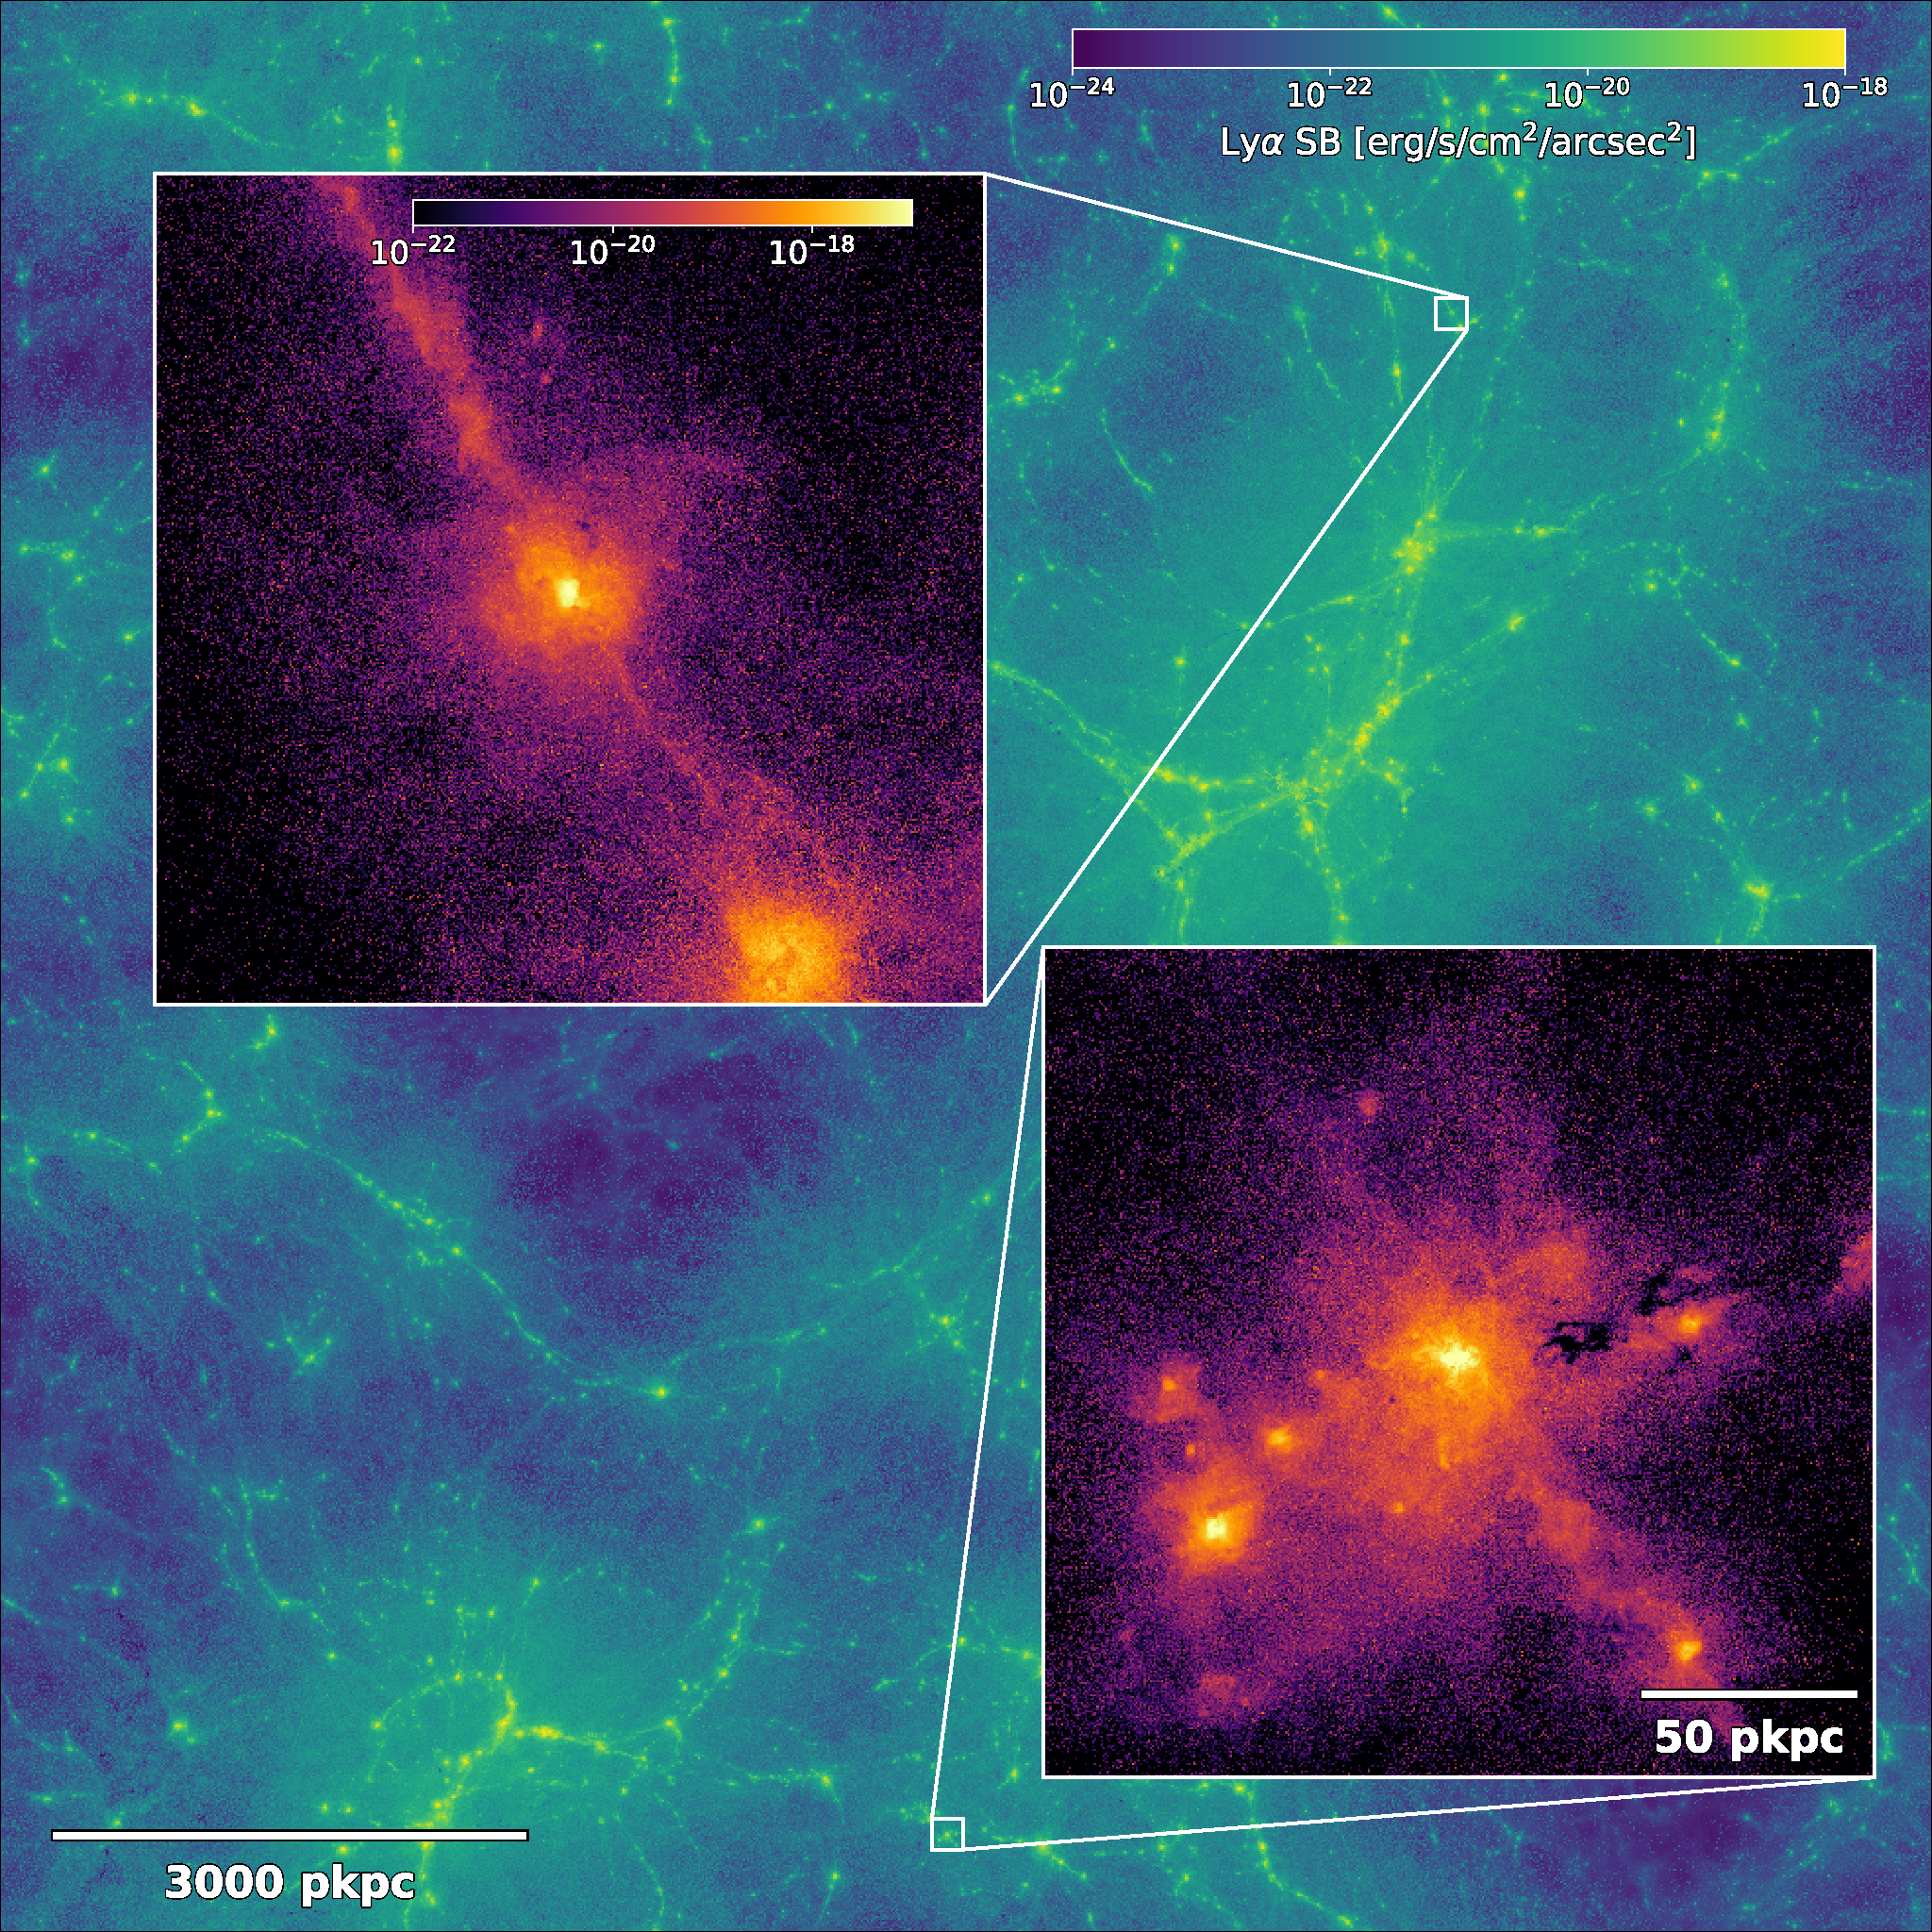
\includegraphics[width=0.7\linewidth]{./pic/TNG50_z3_LymanAlpha_emission_2k.png}
	\caption{}
	\label{fig:TNG50_z3_LymanAlpha_emission_2k}
\end{figure}

Illustrisプロジェクトのシミュレーションを含め,Illustris-TNGプロジェクトのシミュレーションデータは以下の通りが公開されている.

\begin{figure}[H]
	\centering
	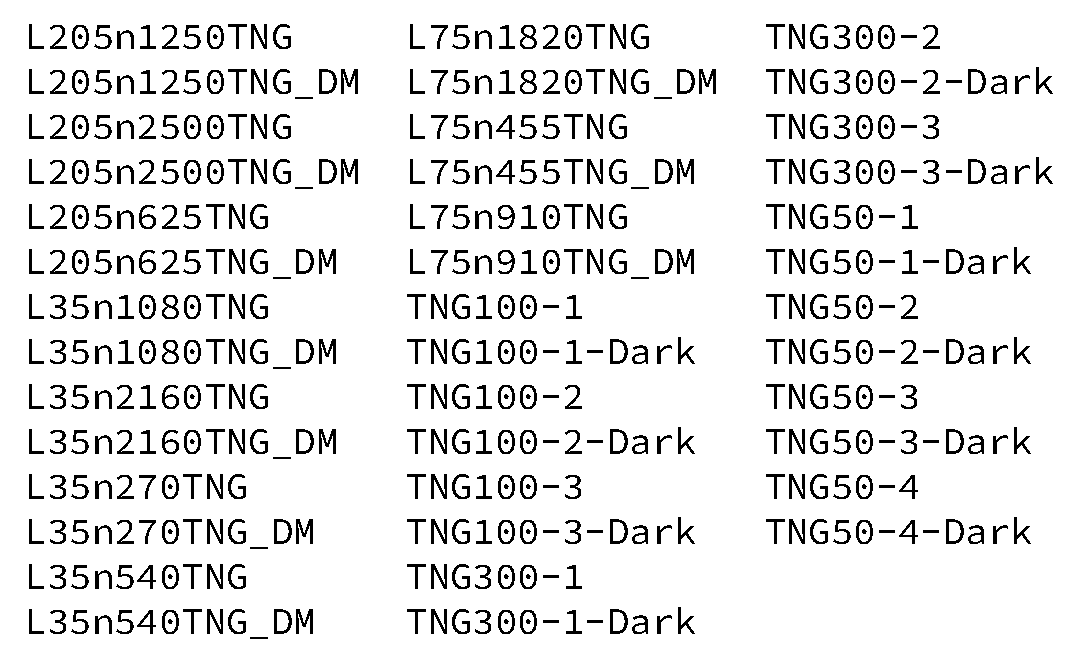
\includegraphics[width=0.5\linewidth]{./pic/ALLsimTNG.pdf}
\end{figure}

シミュレーションデータのディレクトリ下には次のようなディレクトリとファイルが存在する:\texttt{output/},\texttt{processing/},\texttt{simulation.hdf5}

\subsubsection{\texttt{output}ディレクトリ}

\texttt{output/}ディレクトリ下には,グループカタログ,スナップショット,Subboxなどのデータが存在する.グループカタログにはHalo(銀河団)カタログやSubhalo(銀河)カタログが存在する.スナップショットには宇宙誕生を0として,現在を99として100個のスナップショットファイルが存在する.例えばTNG50-1の場合,宇宙誕生から0.179 Gyrをスナップショット0として13.803 Gyrをスナップショット99としている.ディレクトリ「\texttt{groups\_*}」,「\texttt{snapdir\_*}」の\texttt{*}には3桁でスナップショット番号が入る.現在の宇宙(スナップショット99)を使用したい場合は,ディレクトリ「\texttt{groups\_099}」,「\texttt{snapdir\_099}」を見れば良い.

そのディレクトリ下には,グループカタログやスナップショットのデータは大きいため,複数のファイルに分割されていて,これをチャンクファイルという. グループカタログのチャンクファイルは「\texttt{fof\_subhalo\_tab\_*}」もしくは「\texttt{groups\_*}」のファイル名でで定義され連番表記されている.

\subsection{観測対象の選択}

Illustris-TNGには「TNG50 MW/M31-like catalog (天の川銀河に似た銀河のカタログ)」が公開されている\citep{pillepich_milky_2023}.そのうち,Fermi/eROSITA-like bubblesが観測されているsubhaloのカタログが公開されており\citep{pillepich_x-ray_2021},その127個のsubhaloを解析することにする.その一覧を表\ref{tab:virialtable}に示す.このカタログのsubhaloのビリアル半径と質量の分布を図\ref{fig:distribution_of_VR_MASS}に示す。

\begin{figure}
	\centering
	\begin{minipage}[b]{0.45\linewidth}
		\centering
		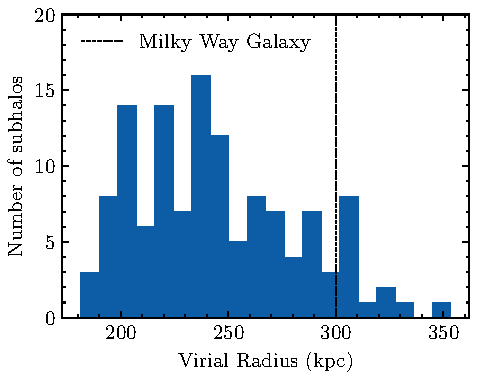
\includegraphics[width=\linewidth]{pic/numsubhalo}
		\subcaption{}
		\label{fig:numsubhalo}
	\end{minipage}
	\begin{minipage}[b]{0.45\linewidth}
		\centering
		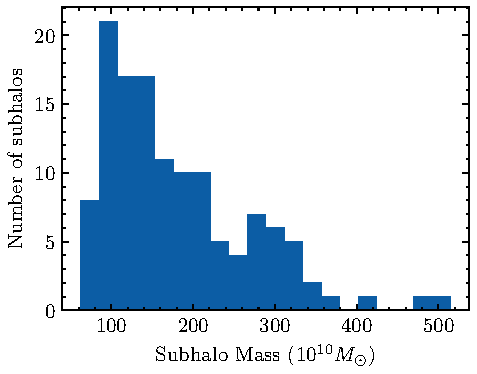
\includegraphics[width=\linewidth]{pic/EstimatedSubhaloMass}
		\subcaption{}
		\label{fig:estimatedsubhalomass}
	\end{minipage}
	\caption{}
	\label{fig:distribution_of_VR_MASS}
\end{figure}

我々の天の川銀河よりもビリアル半径と質量は比較的小さいものが多い。

